\section{学習後に自分側の重みを写す比較の詳細}\label{sup:copy}
学習を終えた非共有条件のモデルで，process-2 用の LSTM に process-1 用の重みを写した（本文3.3節，図\ref{fig:bcopy}）．
快・不快を受ける入力の8列だけを写した場合，他者の位置の追跡は元のままであったが，G5b は3組とも元の非共有条件と同じく0前後で（$-0.035$〜$+0.030$），事前登録した予想は支持されなかった．
自分側で学んだ快・不快の入口の重みだけでは，他者側の働きは戻らなかった．
LSTM の重みをすべて写した場合は，$h^2$ から A-2 の位置を読む決定係数が3組とも基準の 0.8 を下回り（0.60〜0.75），事前登録した基準により，予測画像を通る量（G5b，符号に従う分）は判定できなかった．
経験なし条件の非共有モデルに同じように写しても G5b は大きく動いたので（$+0.10$〜$+0.56$，事前登録外の確認），写したときの予測画像の値は，写した $h^2$ と元の $h^2$ に合わせて学習された視覚予測器との食い違いを強く受けると考えられる．
一方，視覚予測器を通らない他者特徴基準の照合では，すべて写すと BA が 0.75〜0.77 になり，元の非共有条件（0.41〜0.49）より経験80\%条件（0.74〜0.78）に近づいた（最終5点の平均，組1〜3）．
快・不快の列だけを写した場合は 0.45〜0.55 にとどまった．
この回復が写す操作そのものによるものでないかを，経験なし条件の非共有モデルに同じように写して確かめた（事前登録外の確認）．
経験なし条件のモデルにすべて写しても，他者特徴基準の BA は 0.35〜0.52 にとどまり，経験ありに写した場合との差は3組とも正で信頼区間は0を含まなかった（$+0.41$ [$+0.34$, $+0.47$]，$+0.28$ [$+0.23$, $+0.33$]，$+0.25$ [$+0.20$, $+0.29$]）．
自己視界基準では，どの写し方でも差はなかった．
さらに，視覚予測器を通らないもう一つの量として，真値条件の $\Delta$ を写したモデルで測った．
元の非共有条件の $\Delta$ は，快・不快の入口が学習されていないので，経験の有無によらず $\pm0.002$ 以内であった．
経験ありの重みをすべて写すと，A-2 の割合が 0.5 のデータで真値条件の悪化が現れ（緑好みデータで組2 $+0.095$，組3 $+0.081$，組1 $-0.002$），経験なしの重みを写した場合（$-0.054$〜$-0.047$）との差は3組とも二つのデータで正であった．
A-2 の割合を 0.8 にしたときの $\Delta$ の変化も，経験ありの重みを写すと $-0.13$〜$-0.11$ で，共有ありの経験80\%条件（$-0.16$〜$-0.08$）と同じ程度であった．経験なしの重みや快・不快の列だけを写した場合は $-0.05$〜$-0.02$ にとどまった．
ただし，$\Delta$ の値そのものは組ごとには経験80\%条件と一致しなかった．
% 出典：paper_extra_log.md §20（測り方，fbe12c5）・§24（結果，94bf4ea），paper_extra_results_log.md。CPU で測り，GPU の値と丸めの範囲で一致を確認。
% 出典：paper_extra_results_log.md §B，paper_extra_log.md §18（Claude Code，コミット 503efb1）。B1（全部写す）は判定不能，B3（列だけ）は不支持，B2 は記述。
以上から，視覚予測器を通らない二つの量（他者特徴基準の照合と真値条件の $\Delta$）では，学習の後に経験ありの自分側の LSTM 全体を写すと，共有ありの経験80\%条件と同じ形の働きが戻った．
経験なしの重みや，快・不快の入口の重みだけでは戻らなかった．
これは，他者側の働きに要るのは学習中の重みの共有そのものではなく，自分の経験で学んだ計算（LSTM 全体）が他者側で使われることだという考えを支持する．
ただし，この確認は事前登録外であり，予測画像を通る量（G5b，符号に従う分）は写す操作による食い違いのために測れなかった．
また，重ね合わせ機構という仕組みに固有の効果であるとは言えない．
% 出典：v13 まとめ §5（表5，h2→A-2 の位置 R^2，v13 − NS の範囲）。

\begin{figure}[tbp]
  \centering
  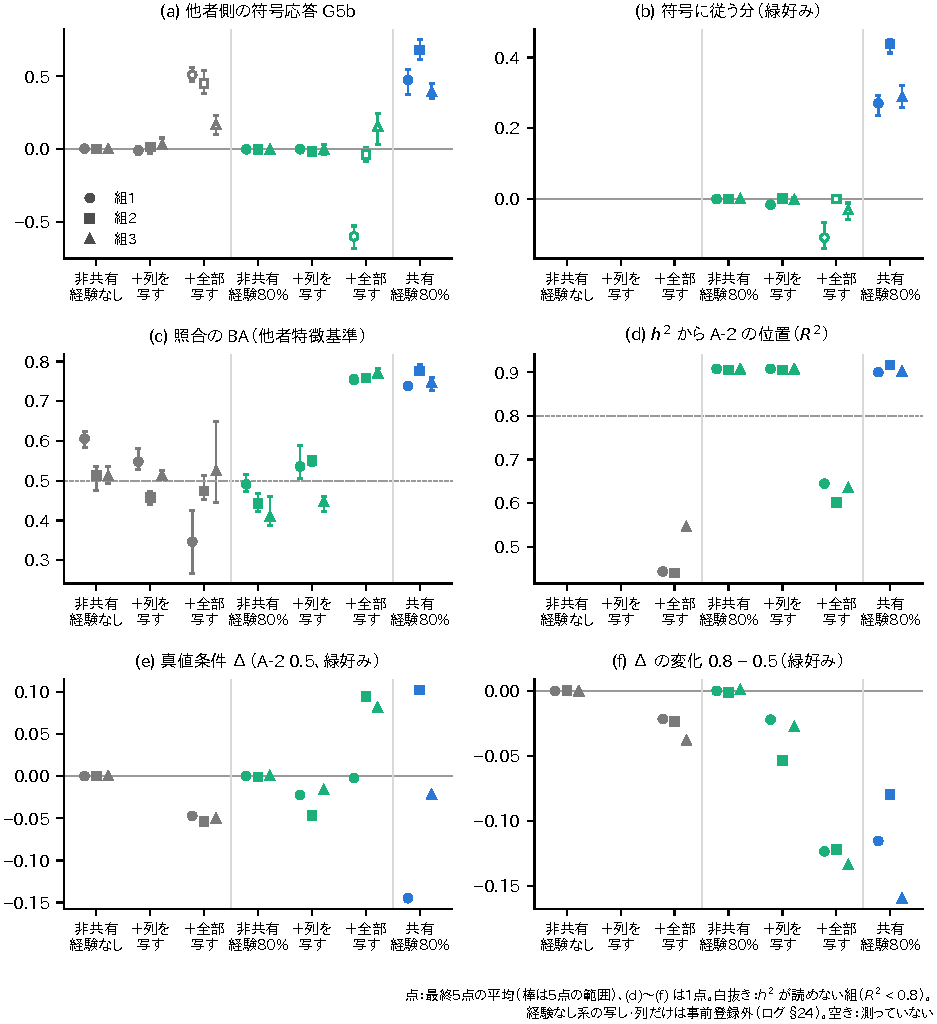
\includegraphics[width=\linewidth]{figs/b_copy}
  % 元：data/result/paper_extra/B_copy/figs/b_copy.pdf
  \caption{学習後に自分側の重みを写す比較．横軸は，非共有条件の経験なし・その列だけ写す・全部写す，非共有条件の経験80\%・その列だけ写す・全部写す，共有ありの経験80\%条件．○□△ は組1〜3．(a) G5b，(b) 符号に従う分，(c) 照合の BA（他者特徴基準），(d) $h^2$ から A-2 の位置を読む決定係数，(e) 真値条件の $\Delta$（A-2 の割合 0.5），(f) A-2 の割合を 0.8 にしたときの $\Delta$ の変化．(a)(b) の白抜きは $h^2$ の読み出しが基準に届かず判定しない組．}
  \label{fig:bcopy}
\end{figure}
